%% Utilizando como base o modelo do abntex2
%% abtex2-modelo-trabalho-academico.tex, v<VERSION> laurocesar
%% Copyright 2012-<COPYRIGHT_YEAR> by abnTeX2 group at http://www.abntex.net.br/ 
%%
%% This work may be distributed and/or modified under the
%% conditions of the LaTeX Project Public License, either version 1.3
%% of this license or (at your option) any later version.
%% The latest version of this license is in
%%   http://www.latex-project.org/lppl.txt
%% and version 1.3 or later is part of all distributions of LaTeX
%% version 2005/12/01 or later.
%%
%% This work has the LPPL maintenance status `maintained'.
%% 
%% The Current Maintainer of this work is the abnTeX2 team, led
%% by Lauro César Araujo. Further information are available on 
%% http://www.abntex.net.br/
%%
%% This work consists of the files abntex2-modelo-trabalho-academico.tex,
%% abntex2-modelo-include-comandos and abntex2-modelo-references.bib
%%

% ------------------------------------------------------------------------
% ------------------------------------------------------------------------
% abnTeX2: Modelo de Trabalho Academico (tese de doutorado, dissertacao de
% mestrado e trabalhos monograficos em geral) em conformidade com 
% ABNT NBR 14724:2011: Informacao e documentacao - Trabalhos academicos -
% Apresentacao
% ------------------------------------------------------------------------
% ------------------------------------------------------------------------

\documentclass[
	% -- opções da classe memoir --
	12pt,				% tamanho da fonte
	openright,			% capítulos começam em pág ímpar (insere página vazia caso preciso)
	oneside,			% para impressão em recto e verso. Oposto a oneside
	a4paper,			% tamanho do papel. 
	% -- opções da classe abntex2 --
	%chapter=TITLE,		% títulos de capítulos convertidos em letras maiúsculas
	%section=TITLE,		% títulos de seções convertidos em letras maiúsculas
	%subsection=TITLE,	% títulos de subseções convertidos em letras maiúsculas
	%subsubsection=TITLE,% títulos de subsubseções convertidos em letras maiúsculas
	% -- opções do pacote babel --
	english,			% idioma adicional para hifenização
	french,				% idioma adicional para hifenização
	spanish,			% idioma adicional para hifenização
	brazil				% o último idioma é o principal do documento
	]{abntex2}

% ---
% Pacotes básicos 
% ---

\usepackage{lmodern}			% Usa a fonte Latin Modern			
\usepackage[T1]{fontenc}		% Selecao de codigos de fonte.
\usepackage[utf8]{inputenc}		% Codificacao do documento (conversão automática dos acentos)
\usepackage{indentfirst}		% Indenta o primeiro parágrafo de cada seção.
\usepackage{color}				% Controle das cores
\usepackage{graphicx}			% Inclusão de gráficos
\usepackage{microtype} 			% para melhorias de justificação
% ---
%\usepackage{float}
\usepackage{longtable}
\usepackage{multirow}
% ---
% Pacotes adicionais, usados apenas no âmbito do Modelo Canônico do abnteX2
% ---
\usepackage{lipsum}				% para geração de dummy text
% ---

% ---
% Pacotes de citações
% ---
\usepackage[alf,abnt-emphasize=bf]{abntex2cite}	% Citações padrão ABNT

% --- 
% CONFIGURAÇÕES DE PACOTES
% --- 

% ---
% Configurações do pacote backref
% Usado sem a opção hyperpageref de backref
\renewcommand{\backrefpagesname}{Citado na(s) página(s):~}
% Texto padrão antes do número das páginas
\renewcommand{\backref}{}
% Define os textos da citação
\renewcommand*{\backrefalt}[4]{
	\ifcase #1 %
		Nenhuma citação no texto.%
	\or
		Citado na página #2.%
	\else
		Citado #1 vezes nas páginas #2.%
	\fi}%
% ---

\newcommand{\quadroname}{Quadro}
\newcommand{\listofquadrosname}{Lista de quadros}

\makeatletter
\setlength{\@fptop}{5pt} % Set distance from top of page to first float
\makeatother
% ---

% ---
% Possibilita criação de Quadros e Lista de quadros.
% Ver https://github.com/abntex/abntex2/issues/176
%


\newfloat[chapter]{quadro}{loq}{\quadroname}
\newlistof{listofquadros}{loq}{\listofquadrosname}
\newlistentry{quadro}{loq}{0}

% configurações para atender às regras da ABNT
\setfloatadjustment{quadro}{\centering}
\counterwithout{quadro}{chapter}
\renewcommand{\cftquadroname}{\quadroname\space} 
\renewcommand*{\cftquadroaftersnum}{\hfill--\hfill}

\newcommand{\citadurante}[2][]{
    \ifx&#1&%
      \citeauthoronline{#2}(\citeyear{#2})
    \else
      \citeauthoronline{#2}(\citeyear{#2}, #1)
    \fi
}
\newcommand{\legenda}[1]{
    \captionnamefont{\footnotesize}
    \captiontitlefont{\footnotesize}
    \caption{#1}
}
\newcommand{\source}[1]{\fonte{#1}}
\newcommand{\paragrafo}{\par}


\setfloatlocations{quadro}{hbtp} % Ver https://github.com/abntex/abntex2/issues/176
% ---

% --- 
% Espaçamentos entre linhas e parágrafos 
% --- 

% O tamanho do parágrafo é dado por:
\setlength{\parindent}{1.3cm}

% Controle do espaçamento entre um parágrafo e outro:
\setlength{\parskip}{0.2cm}  % tente também \onelineskip
\titulo{TÍTULO: subtítulo}
\autor{NOME COMPLETO DO ELABORADOR}
\local{LOCAL}
\data{ANO}
\orientador{Nome do(a) Orientador(a)}
\instituicao{%
  Universidade Federal do Rio Grande do Norte}
\tipotrabalho{Monografia de Gradução}
% O preambulo deve conter o tipo do trabalho, o objetivo, 
% o nome da instituição e a área de concentração 
\preambulo{Monografia apresentada ao Curso de Engenharia de Produção, como requisito para obtenção do Título de Engenheiro de Produção da Universidade Federal do Rio Grande do Norte.\\Orientador:Nome do(a) Orientador(a)}
% ---
% Informações de dados para CAPA e FOLHA DE ROSTO
% ---
% ---


% ---
% Configurações de aparência do PDF final

% alterando o aspecto da cor azul
\definecolor{blue}{RGB}{41,5,195}
\definecolor{black}{RGB}{0,0,0}

% informações do PDF
\makeatletter
\hypersetup{
     	%pagebackref=true,
		pdftitle={\@title}, 
		pdfauthor={\@author},
    	pdfsubject={\imprimirpreambulo},
	    pdfcreator={LaTeX with abnTeX2},
		pdfkeywords={abnt}{latex}{abntex}{abntex2}{trabalho acadêmico}, 
		colorlinks=true,       		% false: boxed links; true: colored links
    	linkcolor=black,          	% color of internal links
    	citecolor=black,        		% color of links to bibliography
    	filecolor=black,      		% color of file links
		urlcolor=black,
		bookmarksdepth=4
}
\makeatother
% --- 

% ---
% Posiciona figuras e tabelas no topo da página quando adicionadas sozinhas
% em um página em branco. Ver https://github.com/abntex/abntex2/issues/170

% aqui comandos

% ---
% compila o indice
% ---
%\makeindex
% ---

% ----
% Início do documento
% ----
\usepackage{float}
\usepackage{pdfpages}
\begin{document}

% Seleciona o idioma do documento (conforme pacotes do babel)
%\selectlanguage{english}
\selectlanguage{brazil}

% Retira espaço extra obsoleto entre as frases.
\frenchspacing 

% ----------------------------------------------------------
% ELEMENTOS PRÉ-TEXTUAIS
% ----------------------------------------------------------
% \pretextual

% ---
% Capa
% ---
% alterando a capa
\renewcommand{\imprimircapa}{%
  \begin{capa}%
    \center
    {\ABNTEXchapterfont\Large Universidade Federal do Rio Grande do Norte}
    \vspace*{0.5cm}\\
    {\ABNTEXchapterfont\Large Curso de Engenharia de Produção}
    \vspace*{0.5cm}\\
    {\ABNTEXchapterfont\large\imprimirautor}

    \vfill
    \begin{center}
    \ABNTEXchapterfont\bfseries\LARGE\imprimirtitulo
    \end{center}
    \vfill
    
    \large\imprimirlocal

    \large\imprimirdata
    
    \vspace*{1cm}
  \end{capa}
}

\imprimircapa
% ---

% ---
% Folha de rosto
% (o * indica que haverá a ficha bibliográfica)
% ---
% Anverso
\imprimirfolhaderosto*

\begin{fichacatalografica}
    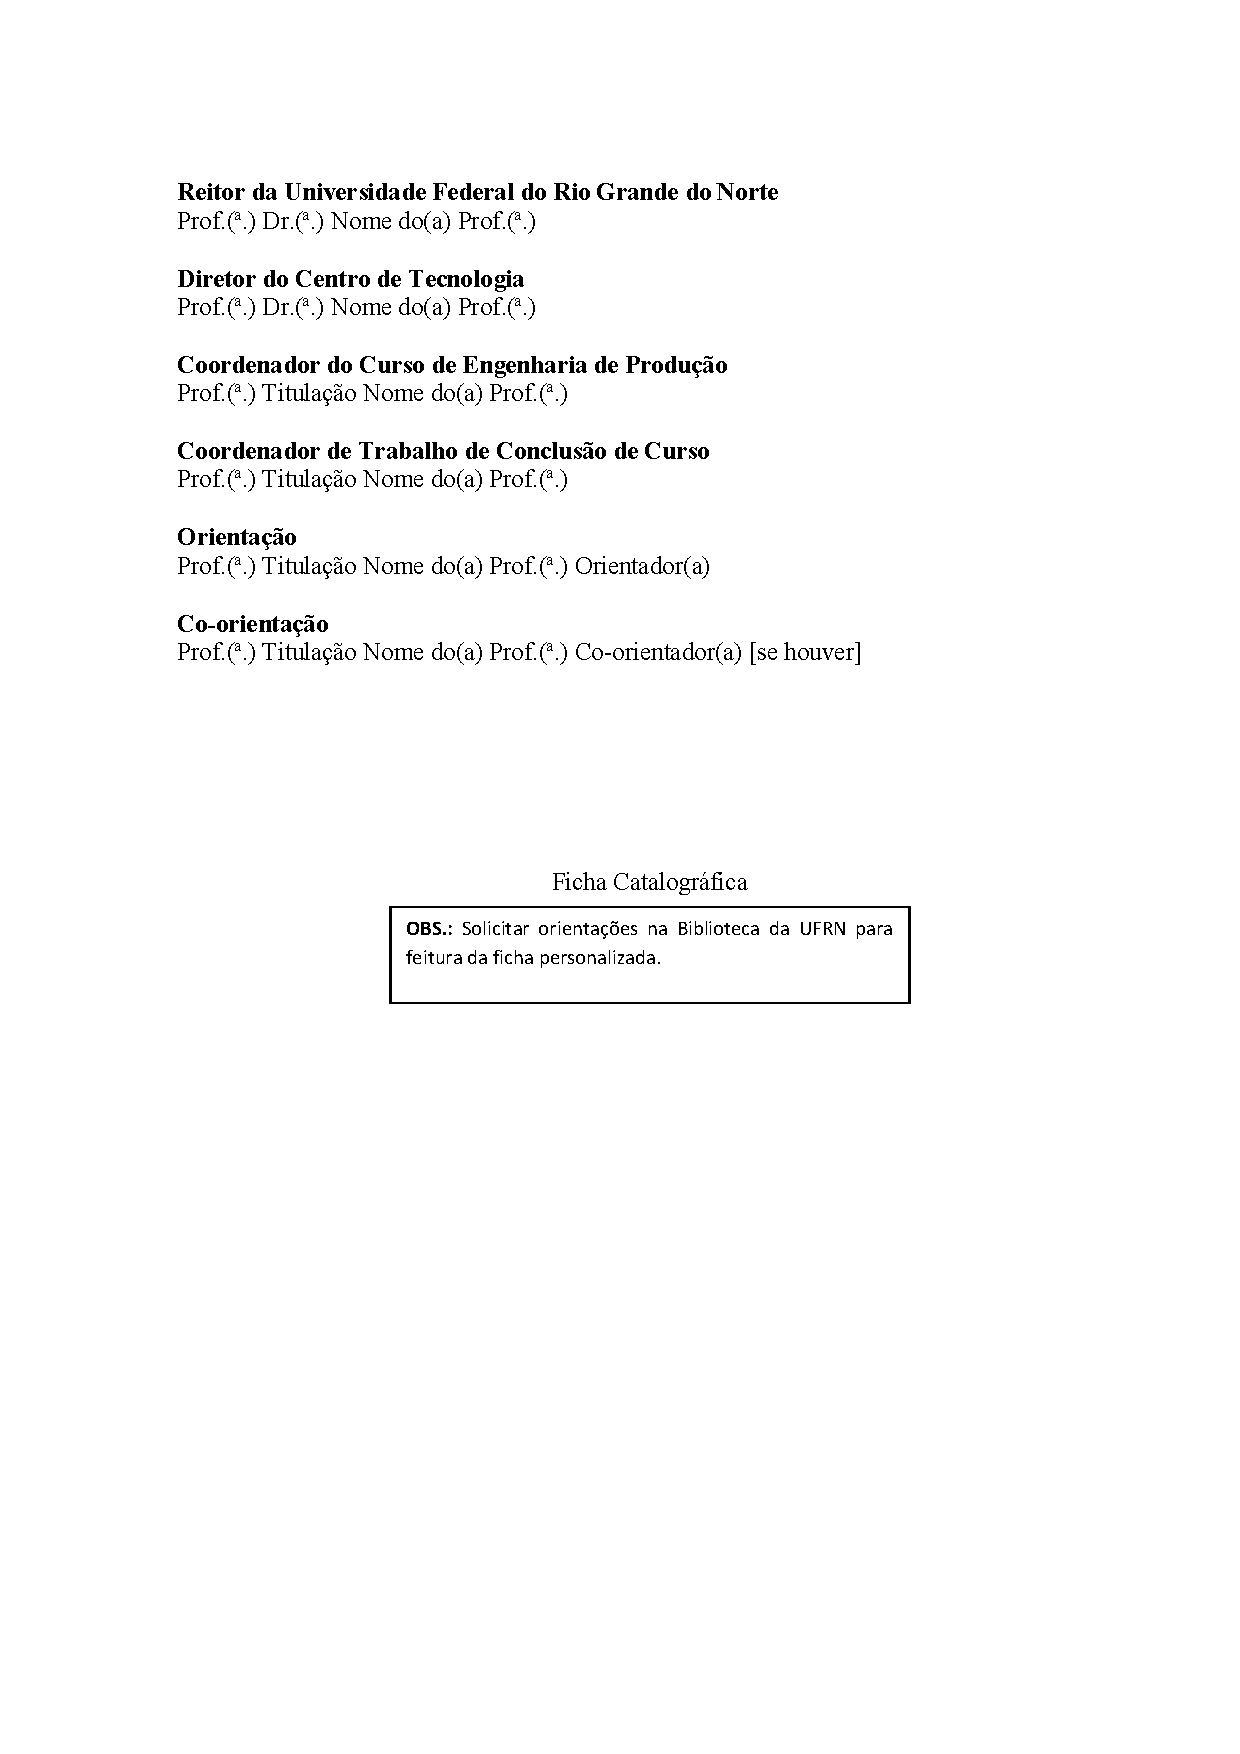
\includepdf[pages=-]{ficha.pdf}
\end{fichacatalografica}
% Verso
%\begin{fichacatalografica}
%	\sffamily
%	\vspace*{\fill}					% Posição vertical
%	\begin{center}					% Minipage Centralizado
%	\fbox{\begin{minipage}[c][8cm]{13.5cm}		% Largura
%	\small
%	
%	Sobrenome, Nome do autor
	
%	\hspace{0.5cm} \imprimirtitulo  / \imprimirautor. --
%	\imprimirlocal, \imprimirdata-
	
%	\hspace{0.5cm} \thelastpage p. : il. (algumas color.) ; 30 cm.\\
	
%	\hspace{0.5cm} \imprimirorientadorRotulo~\imprimirorientador\\
	
%	\hspace{0.5cm}
%	\parbox[t]{\textwidth}{\imprimirtipotrabalho~--~\imprimirinstituicao,
%	\imprimirdata.}\\
	
%	\hspace{0.5cm}
%		1. Palavra 1.
%		2. Palavra 2.
%		3. Palavra 3.
%		4. Palavra 4.
%		5. Palavra 5.
%		6. Palavra 6.
%		I. Orientador.
%		II. Universidade Federal do Rio Grande do Norte.
%		III. Departamento de Engenharia de Produção.
%		IV. Título			
%	\end{minipage}}
%	\end{center}
%\end{fichacatalografica}
% ---

% ---
% Inserir a ficha bibliografica
% ---

% Isto é um exemplo de Ficha Catalográfica, ou ``Dados internacionais de
% catalogação-na-publicação''. Você pode utilizar este modelo como referência. 
% Porém, provavelmente a biblioteca da sua universidade lhe fornecerá um PDF
% com a ficha catalográfica definitiva após a defesa do trabalho. Quando estiver
% com o documento, salve-o como PDF no diretório do seu projeto e substitua todo
% o conteúdo de implementação deste arquivo pelo comando abaixo:
%
%\begin{fichacatalografica}
%     \includepdf{fig_ficha_catalografica.pdf}
%\end{fichacatalografica}
% ---

% ---
% Inserir errata
% ---
\begin{errata}
Elemento opcional da \citeonline[4.2.1.2]{NBR14724:2011}. Exemplo:

\vspace{\onelineskip}

FERRIGNO, C. R. A. \textbf{Tratamento de neoplasias ósseas apendiculares com
reimplantação de enxerto ósseo autólogo autoclavado associado ao plasma
rico em plaquetas}: estudo crítico na cirurgia de preservação de membro em
cães. 2011. 128 f. Tese (Livre-Docência) - Faculdade de Medicina Veterinária e
Zootecnia, Universidade de São Paulo, São Paulo, 2011.

\begin{table}[htb]
\center
\footnotesize
\begin{tabular}{|p{1.4cm}|p{1cm}|p{3cm}|p{3cm}|}
  \hline
   \textbf{Folha} & \textbf{Linha}  & \textbf{Onde se lê}  & \textbf{Leia-se}  \\
    \hline
    1 & 10 & auto-conclavo & autoconclavo\\
   \hline
\end{tabular}
\end{table}

\end{errata}
% ---

% ---
% Inserir folha de aprovação
% ---

% Isto é um exemplo de Folha de aprovação, elemento obrigatório da NBR
% 14724/2011 (seção 4.2.1.3). Você pode utilizar este modelo até a aprovação
% do trabalho. Após isso, substitua todo o conteúdo deste arquivo por uma
% imagem da página assinada pela banca com o comando abaixo:
%
% \begin{folhadeaprovacao}
% \includepdf{folhadeaprovacao_final.pdf}
% \end{folhadeaprovacao}
%
%Folha externa

\begin{folhadeaprovacao}
 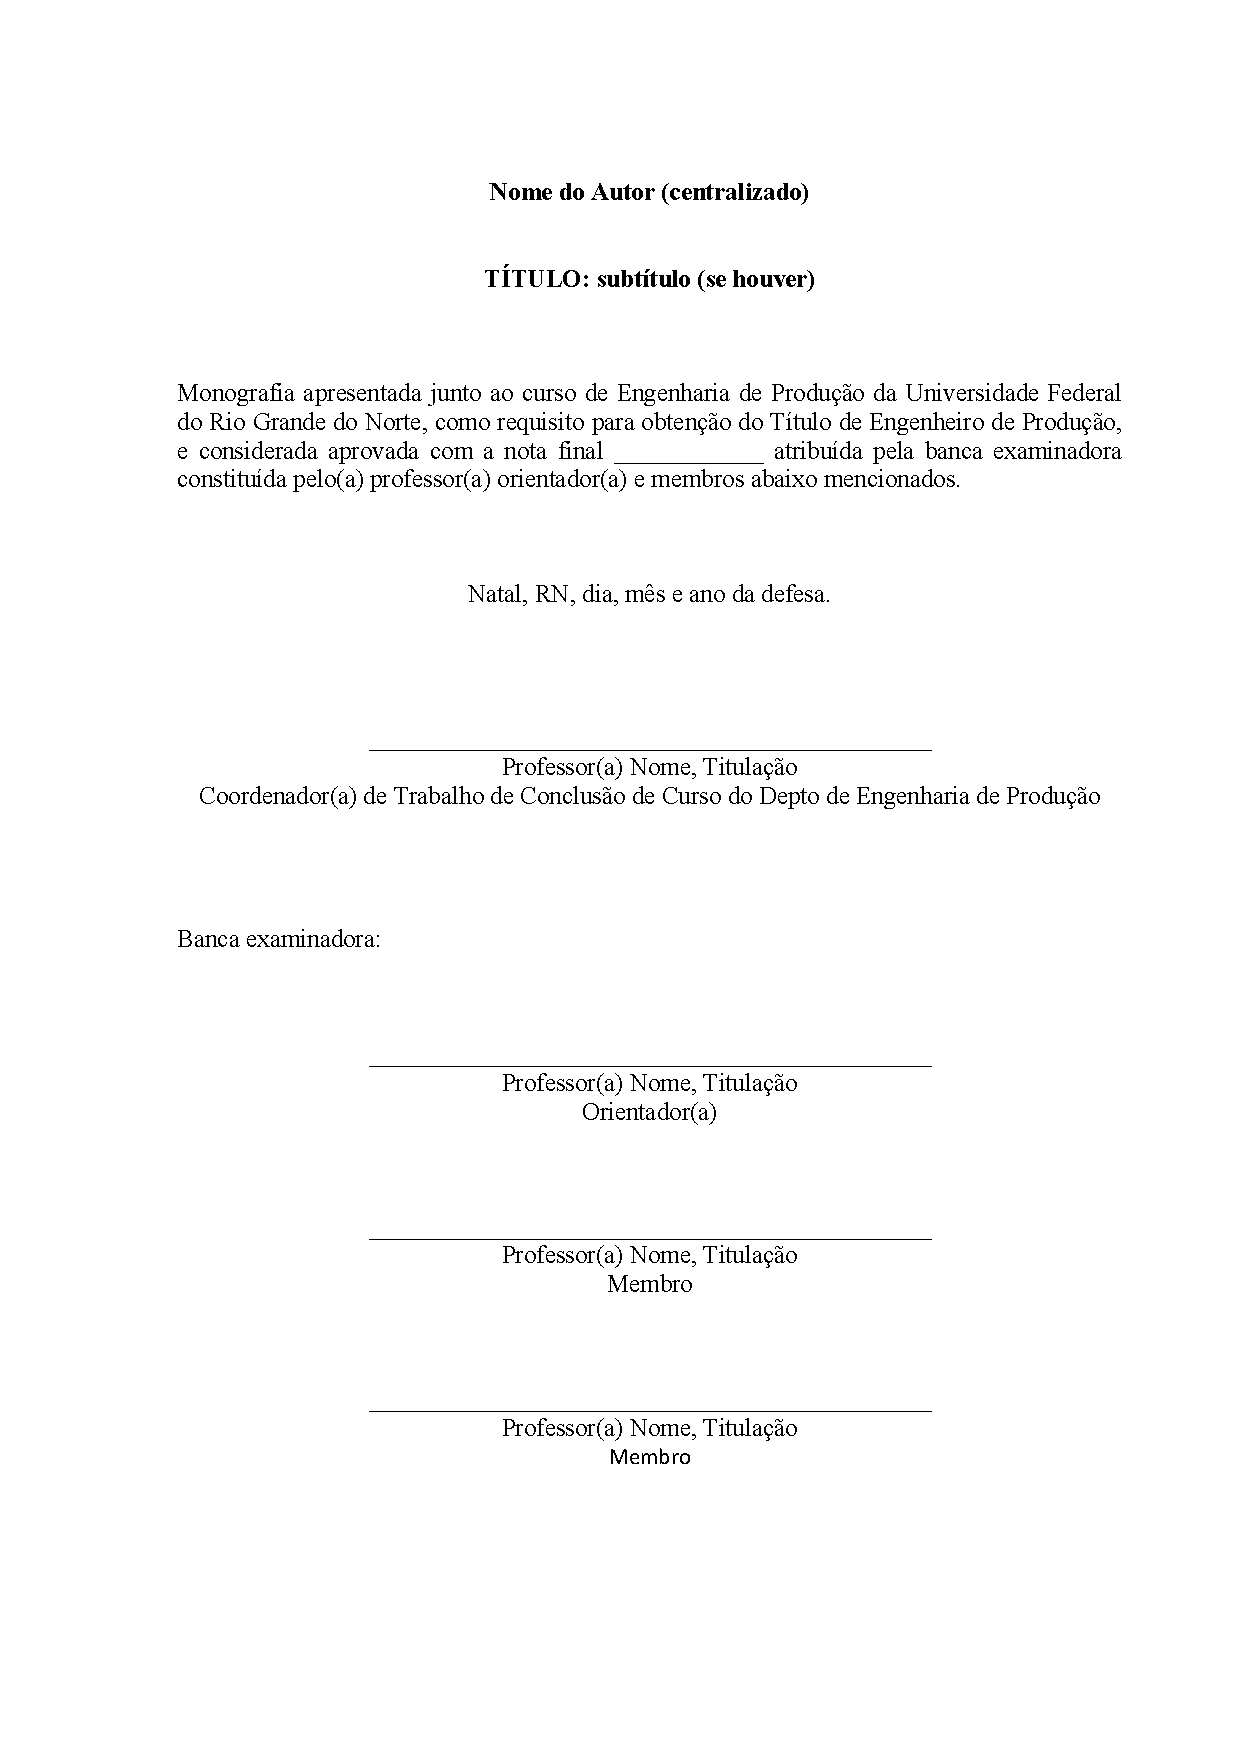
\includepdf[pages=-]{ata.pdf}
\end{folhadeaprovacao}
% ---

% ---
% Dedicatória
% ---
\begin{dedicatoria}
   \vspace*{\fill}
   \centering
   \noindent
   \textit{(relações pessoais)} \vspace*{\fill}
\end{dedicatoria}
% ---
% ---
% Agradecimentos
% ---
\begin{agradecimentos}
\paragrafo{}
Relação das pessoas importantes para a elaboração da monografia.
\paragrafo{}
Exemplos: 
\paragrafo{}
Ao professor 
\paragrafo{}
Aos amigos
\paragrafo{}
Aos trabalhadores da empresa 
\paragrafo{}
Aos Parentes
\end{agradecimentos}
% ---

% ---
% Epígrafe
% ---
\begin{epigrafe}
    \vspace*{\fill}
	\begin{flushright}
		\textit{Normalmente uma citação que represente\\
			    o estado do autor com relação ao trabalho.}
	\end{flushright}
\end{epigrafe}
% ---
% ---
% RESUMOS
% ---
% resumo em português
\setlength{\absparsep}{18pt} % ajusta o espaçamento dos parágrafos do resumo
\begin{resumo}
Texto de, aproximadamente, dez linhas ou trezentas palavras, não podendo ultrapassar uma página, em que faz-se uma breve apresentação do estudo realizado, informando: tipo de abordagem, métodos e restrições do estudo, material utilizado, sustentação teórica, delimitação do tema, caso haja pesquisa de campo, onde foi realizada e, ainda, indicação das conclusões obtidas\\
 \textbf{Palavras-chave}: palavra 1, palavra 2, até 5 palavras.
\end{resumo}
% resumo em inglês
\begin{resumo}[Abstract]
 \begin{otherlanguage*}{english}
   Versão inglês do texto correspondente ao RESUMO de aproximadamente dez linhas ou trezentas palavras, não podendo ultrapassar uma página.\\
   \noindent 
   \textbf{Keywords}: versão em inglês das palavras chaves.
 \end{otherlanguage*}
\end{resumo}
% ---
% ---
% inserir lista de ilustrações
% ---
\pdfbookmark[0]{\listfigurename}{lof}
\listoffigures*
\cleardoublepage
% ---
% ---
% inserir lista de quadros
% ---
\pdfbookmark[0]{\listofquadrosname}{loq}
\listofquadros*
\cleardoublepage
% ---
% ---
% inserir lista de tabelas
% ---
\pdfbookmark[0]{\listtablename}{lot}
\listoftables*
\cleardoublepage
% ---
% ---
% inserir lista de abreviaturas e siglas
% ---
\begin{siglas}
  \item[ABNT] Associação Brasileira de Normas Técnicas
  \item[abnTeX] ABsurdas Normas para TeX
  \item[UFRN] Universidade Federal do Rio Grande do Norte
\end{siglas}
% ---
% ---
% inserir lista de símbolos
% ---
\begin{simbolos}
  \item[$ \Gamma $] Letra grega Gama
  \item[$ \Lambda $] Lambda
  \item[$ \zeta $] Letra grega minúscula zeta
  \item[$ \in $] Pertence
\end{simbolos}
% ---
% ---
% inserir o sumario
% ---
\pdfbookmark[0]{\contentsname}{toc}
\tableofcontents*
\cleardoublepage
% ---
% ----------------------------------------------------------
% ELEMENTOS TEXTUAIS
% ----------------------------------------------------------
\textual
% ----------------------------------------------------------
% Introdução (exemplo de capítulo sem numeração, mas presente no Sumário)
% ----------------------------------------------------------
\chapter{Introdução}
%%
%% Capítulo 1: Modelo de Capítulo
%%

% Está sendo usando o comando \mychapter, que foi definido no arquivo
% comandos.tex. Este comando \mychapter é essencialmente o mesmo que o
% comando \chapter, com a diferença que acrescenta um \thispagestyle{empty}
% após o \chapter. Isto é necessário para corrigir um erro de LaTeX, que
% coloca um número de página no rodapé de todas as páginas iniciais dos
% capítulos, mesmo quando o estilo de numeração escolhido é outro.
\paragrafo{}
Texto Texto Texto Texto Texto Texto Texto Texto Texto Texto Texto Texto Texto Texto Texto Texto Texto Texto Texto Texto Texto Texto Texto Texto Texto Texto Texto Texto Texto Texto Texto Texto Texto Texto Texto Texto Texto Texto Texto Texto Texto Texto. 
\section{Apresentação}
\label{apresentacao}
\paragrafo{}
Texto Texto Texto Texto Texto Texto Texto Texto Texto Texto Texto Texto Texto Texto Texto Texto Texto Texto Texto Texto Texto Texto Texto Texto Texto Texto Texto Texto Texto Texto Texto Texto Texto Texto Texto Texto Texto Texto Texto Texto Texto Texto. 
\paragrafo{}
Texto Texto Texto Texto Texto Texto Texto Texto Texto Texto Texto Texto Texto Texto Texto Texto Texto Texto Texto Texto Texto Texto Texto Texto Texto Texto Texto Texto Texto Texto Texto Texto Texto Texto Texto Texto Texto Texto Texto Texto Texto Texto. 
\section{Objetivos}
\label{objetivo}
\subsection{Objetivo Geral}
\paragrafo{}
Texto Texto Texto Texto Texto Texto Texto Texto Texto Texto Texto Texto Texto Texto Texto Texto Texto Texto Texto Texto Texto Texto Texto Texto Texto Texto Texto Texto Texto Texto Texto Texto Texto Texto Texto Texto Texto Texto Texto Texto Texto Texto.
\subsection{Objetivos Específicos}

\begin{itemize}
  \item \textbf{Objetivo específico 1} : Texto Texto Texto Texto Texto Texto Texto Texto Texto Texto Texto Texto Texto.
  \item \textbf{Objetivo específico 2} : Texto Texto Texto Texto Texto Texto Texto Texto Texto Texto Texto Texto Texto.
  \item \textbf{Objetivo específico 3} : Texto Texto Texto Texto Texto Texto Texto Texto Texto Texto Texto Texto Texto.
\end{itemize}
\section{Justificativa}
\label{justificativa}
\paragrafo{}
Texto Texto Texto Texto Texto Texto Texto Texto Texto Texto Texto Texto Texto Texto Texto Texto Texto Texto Texto Texto Texto Texto Texto Texto Texto Texto Texto Texto Texto Texto Texto Texto Texto Texto Texto Texto Texto Texto Texto Texto Texto Texto.
\paragrafo{}
Texto Texto Texto Texto Texto Texto Texto Texto Texto Texto Texto Texto Texto Texto Texto Texto Texto Texto Texto Texto Texto Texto Texto Texto Texto Texto Texto Texto Texto Texto Texto Texto Texto Texto Texto Texto Texto Texto Texto Texto Texto Texto.

\section{Estrutura dos Capítulos}
\label{estrutura}
\paragrafo{}
Texto Texto Texto Texto Texto Texto Texto Texto Texto Texto Texto Texto Texto Texto Texto Texto Texto Texto Texto Texto Texto Texto Texto Texto Texto Texto Texto Texto Texto Texto Texto Texto Texto Texto Texto Texto Texto Texto Texto Texto Texto Texto.
\paragrafo{}
Texto Texto Texto Texto Texto Texto Texto Texto Texto Texto Texto Texto Texto Texto Texto Texto Texto Texto Texto Texto Texto Texto Texto Texto Texto Texto Texto Texto Texto Texto Texto Texto Texto Texto Texto Texto Texto Texto Texto Texto Texto Texto.
\paragrafo{}
Texto Texto Texto Texto Texto Texto Texto Texto Texto Texto Texto Texto Texto Texto Texto Texto Texto Texto Texto Texto Texto Texto Texto Texto Texto Texto Texto Texto Texto Texto Texto Texto Texto Texto Texto Texto Texto Texto Texto Texto Texto Texto.
 \begin{figure}[H]
    \begin{center}
      % fbox faz uma borda ao redor do seu argumento
		\legenda{Exemplo de Imagem com Latex}
		\fbox{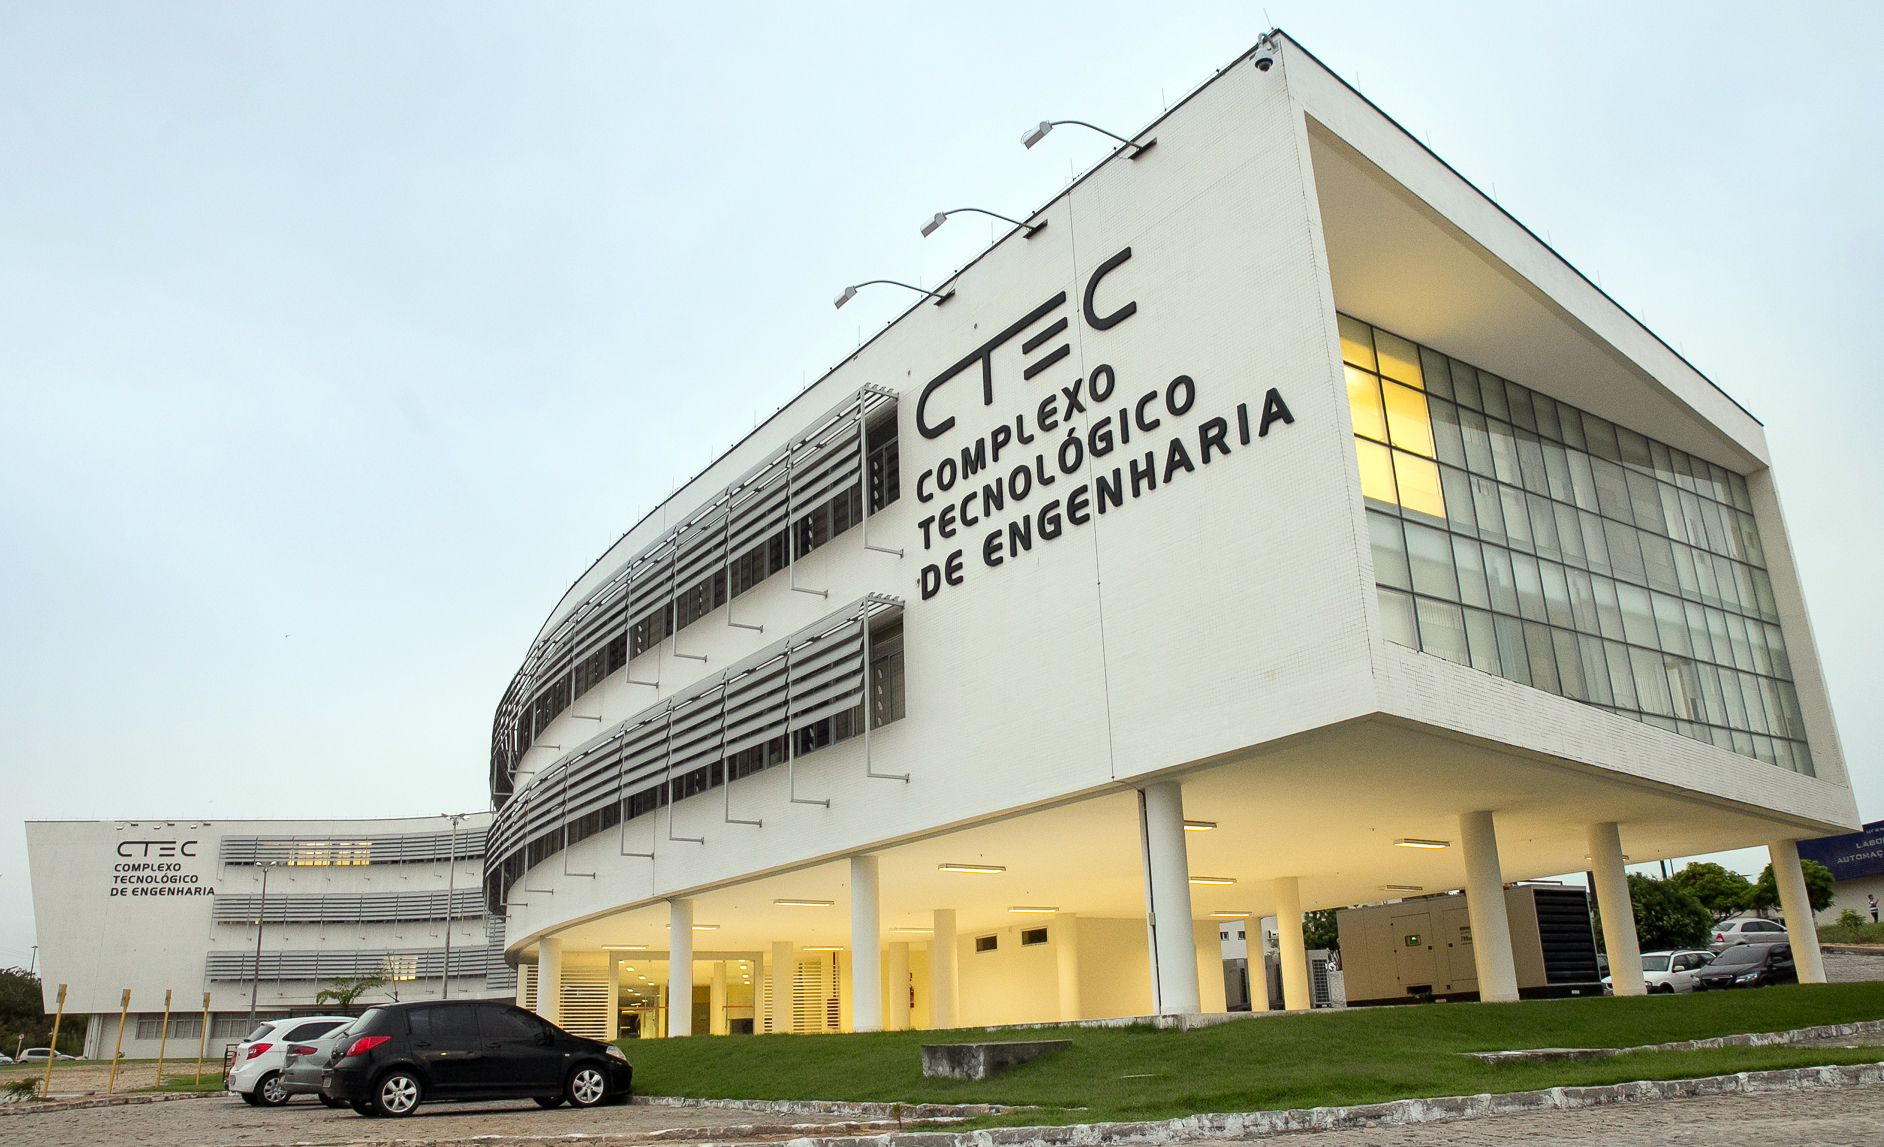
\includegraphics[width=0.95\linewidth]{internos/textuais/capitulo1-introducao/figuras/ctec.jpg}}
		\source{Internet}
		\label{Fig:exemplo1}
	\end{center}
\end{figure}

\chapter{Fundamentação Teórica}
% ----------------------------------------------------------
\paragrafo{}
exemplo de citação na linha \citeonline{MetodologiaYin}, citação de fim de paragrafo \cite{MetodologiaYin}.

\paragrafo{}
Texto Texto Texto Texto Texto Texto Texto Texto Texto Texto Texto Texto Texto Texto Texto Texto Texto Texto Texto Texto Texto Texto Texto Texto Texto Texto Texto Texto Texto Texto Texto Texto Texto Texto Texto Texto Texto Texto Texto Texto Texto Texto.
\paragrafo{}
Texto Texto Texto Texto Texto Texto Texto Texto Texto Texto Texto Texto Texto Texto Texto Texto Texto Texto Texto Texto Texto Texto Texto Texto Texto Texto Texto Texto Texto Texto Texto Texto Texto Texto Texto Texto Texto Texto Texto Texto Texto Texto.
\paragrafo{}
Texto Texto Texto Texto Texto Texto Texto Texto Texto Texto Texto Texto Texto Texto Texto Texto Texto Texto Texto Texto Texto Texto Texto Texto Texto Texto Texto Texto Texto Texto Texto Texto Texto Texto Texto Texto Texto Texto Texto Texto Texto Texto.
\paragrafo{}
Texto Texto Texto Texto Texto Texto Texto Texto Texto Texto Texto Texto Texto Texto Texto Texto Texto Texto Texto Texto Texto Texto Texto Texto Texto Texto Texto Texto Texto Texto Texto Texto Texto Texto Texto Texto Texto Texto Texto Texto Texto Texto.
\paragrafo{}
Texto Texto Texto Texto Texto Texto Texto Texto Texto Texto Texto Texto Texto Texto Texto Texto Texto Texto Texto Texto Texto Texto Texto Texto Texto Texto Texto Texto Texto Texto Texto Texto Texto Texto Texto Texto Texto Texto Texto Texto Texto Texto.
\paragrafo{}
Texto Texto Texto Texto Texto Texto Texto Texto Texto Texto Texto Texto Texto Texto Texto Texto Texto Texto Texto Texto Texto Texto Texto Texto Texto Texto Texto Texto Texto Texto Texto Texto Texto Texto Texto Texto Texto Texto Texto Texto Texto Texto.

\section{Exemplo 1}
\label{exemplo1}
\paragrafo{}
Texto Texto Texto Texto Texto Texto Texto Texto Texto Texto Texto Texto Texto Texto Texto Texto Texto Texto Texto Texto Texto Texto Texto Texto Texto Texto Texto Texto Texto Texto Texto Texto Texto Texto Texto Texto Texto Texto Texto Texto Texto Texto.
\paragrafo{}
Texto Texto Texto Texto Texto Texto Texto Texto Texto Texto Texto Texto Texto Texto Texto Texto Texto Texto Texto Texto Texto Texto Texto Texto Texto Texto Texto Texto Texto Texto Texto Texto Texto Texto Texto Texto Texto Texto Texto Texto Texto Texto.
\paragrafo{}
Texto Texto Texto Texto Texto Texto Texto Texto Texto Texto Texto Texto Texto Texto Texto Texto Texto Texto Texto Texto Texto Texto Texto Texto Texto Texto Texto Texto Texto Texto Texto Texto Texto Texto Texto Texto Texto Texto Texto Texto Texto Texto.
\paragrafo{}
Texto Texto Texto Texto Texto Texto Texto Texto Texto Texto Texto Texto Texto Texto Texto Texto Texto Texto Texto Texto Texto Texto Texto Texto Texto Texto Texto Texto Texto Texto Texto Texto Texto Texto Texto Texto Texto Texto Texto Texto Texto Texto.
\paragrafo{}
Texto Texto Texto Texto Texto Texto Texto Texto Texto Texto Texto Texto Texto Texto Texto Texto Texto Texto Texto Texto Texto Texto Texto Texto Texto Texto Texto Texto Texto Texto Texto Texto Texto Texto Texto Texto Texto Texto Texto Texto Texto Texto.
\paragrafo{}
Texto Texto Texto Texto Texto Texto Texto Texto Texto Texto Texto Texto Texto Texto Texto Texto Texto Texto Texto Texto Texto Texto Texto Texto Texto Texto Texto Texto Texto Texto Texto Texto Texto Texto Texto Texto Texto Texto Texto Texto Texto Texto.
\paragrafo{}
Texto Texto Texto Texto Texto Texto Texto Texto Texto Texto Texto Texto Texto Texto Texto Texto Texto Texto Texto Texto Texto Texto Texto Texto Texto Texto Texto Texto Texto Texto Texto Texto Texto Texto Texto Texto Texto Texto Texto Texto Texto Texto.
\paragrafo{}
Texto Texto Texto Texto Texto Texto Texto Texto Texto Texto Texto Texto Texto Texto Texto Texto Texto Texto Texto Texto Texto Texto Texto Texto Texto Texto Texto Texto Texto Texto Texto Texto Texto Texto Texto Texto Texto Texto Texto Texto Texto Texto.
\paragrafo{}
Texto Texto Texto Texto Texto Texto Texto Texto Texto Texto Texto Texto Texto Texto Texto Texto Texto Texto Texto Texto Texto Texto Texto Texto Texto Texto Texto Texto Texto Texto Texto Texto Texto Texto Texto Texto Texto Texto Texto Texto Texto Texto.
\paragrafo{}
Texto Texto Texto Texto Texto Texto Texto Texto Texto Texto Texto Texto Texto Texto Texto Texto Texto Texto Texto Texto Texto Texto Texto Texto Texto Texto Texto Texto Texto Texto Texto Texto Texto Texto Texto Texto Texto Texto Texto Texto Texto Texto.

\section{Exemplo 2}
\label{exemplo2}
\paragrafo{}
Texto Texto Texto Texto Texto Texto Texto Texto Texto Texto Texto Texto Texto Texto Texto Texto Texto Texto Texto Texto Texto Texto Texto Texto Texto Texto Texto Texto Texto Texto Texto Texto Texto Texto Texto Texto Texto Texto Texto Texto Texto Texto.
\paragrafo{}
Exemplo de equação

  \begin{equation}
  \label{eq:VExperado}
  V = \sum_{i\in{N}} p_{i}	\times V_{i}
  \end{equation}
\paragrafo{}
Texto Texto Texto Texto Texto Texto Texto Texto Texto Texto Texto Texto Texto Texto Texto Texto Texto Texto Texto Texto Texto Texto Texto Texto Texto Texto Texto Texto Texto Texto Texto Texto Texto Texto Texto Texto Texto Texto Texto Texto Texto Texto.
\subsection{Exemplo de Input de Outro arquivo de Texto}
\paragrafo{}
Texto Texto Texto Texto Texto Texto Texto Texto Texto Texto Texto Texto Texto Texto Texto Texto Texto Texto Texto Texto Texto Texto Texto Texto Texto Texto Texto Texto Texto Texto Texto Texto Texto Texto Texto Texto Texto Texto Texto Texto Texto Texto.
\paragrafo{}
Texto Texto Texto Texto Texto Texto Texto Texto Texto Texto Texto Texto Texto Texto Texto Texto Texto Texto Texto Texto Texto Texto Texto Texto Texto Texto Texto Texto Texto Texto Texto Texto Texto Texto Texto Texto Texto Texto Texto Texto Texto Texto.
\paragrafo{}
Texto Texto Texto Texto Texto Texto Texto Texto Texto Texto Texto Texto Texto Texto Texto Texto Texto Texto Texto Texto Texto Texto Texto Texto Texto Texto Texto Texto Texto Texto Texto Texto Texto Texto Texto Texto Texto Texto Texto Texto Texto Texto.
\paragrafo{}
Texto Texto Texto Texto Texto Texto Texto Texto Texto Texto Texto Texto Texto Texto Texto Texto Texto Texto Texto Texto Texto Texto Texto Texto Texto Texto Texto Texto Texto Texto Texto Texto Texto Texto Texto Texto Texto Texto Texto Texto Texto Texto.
\paragrafo{}
Texto Texto Texto Texto Texto Texto Texto Texto Texto Texto Texto Texto Texto Texto Texto Texto Texto Texto Texto Texto Texto Texto Texto Texto Texto Texto Texto Texto Texto Texto Texto Texto Texto Texto Texto Texto Texto Texto Texto Texto Texto Texto.
\paragrafo{}
Texto Texto Texto Texto Texto Texto Texto Texto Texto Texto Texto Texto Texto Texto Texto Texto Texto Texto Texto Texto Texto Texto Texto Texto Texto Texto Texto Texto Texto Texto Texto Texto Texto Texto Texto Texto Texto Texto Texto Texto Texto Texto.
\paragrafo{}
Texto Texto Texto Texto Texto Texto Texto Texto Texto Texto Texto Texto Texto Texto Texto Texto Texto Texto Texto Texto Texto Texto Texto Texto Texto Texto Texto Texto Texto Texto Texto Texto Texto Texto Texto Texto Texto Texto Texto Texto Texto Texto.
\paragrafo{}
Texto Texto Texto Texto Texto Texto Texto Texto Texto Texto Texto Texto Texto Texto Texto Texto Texto Texto Texto Texto Texto Texto Texto Texto Texto Texto Texto Texto Texto Texto Texto Texto Texto Texto Texto Texto Texto Texto Texto Texto Texto Texto.
\paragrafo{}
Texto Texto Texto Texto Texto Texto Texto Texto Texto Texto Texto Texto Texto Texto Texto Texto Texto Texto Texto Texto Texto Texto Texto Texto Texto Texto Texto Texto Texto Texto Texto Texto Texto Texto Texto Texto Texto Texto Texto Texto Texto Texto.
\paragrafo{}
Texto Texto Texto Texto Texto Texto Texto Texto Texto Texto Texto Texto Texto Texto Texto Texto Texto Texto Texto Texto Texto Texto Texto Texto Texto Texto Texto Texto Texto Texto Texto Texto Texto Texto Texto Texto Texto Texto Texto Texto Texto Texto.
\paragrafo{}
Texto Texto Texto Texto Texto Texto Texto Texto Texto Texto Texto Texto Texto Texto Texto Texto Texto Texto Texto Texto Texto Texto Texto Texto Texto Texto Texto Texto Texto Texto Texto Texto Texto Texto Texto Texto Texto Texto Texto Texto Texto Texto.

 

\chapter{Procedimentos e Métodos}
% ----------------------------------------------------------
\paragrafo{}
Texto Texto Texto Texto Texto Texto Texto Texto Texto Texto Texto Texto Texto Texto Texto Texto Texto Texto Texto Texto Texto Texto Texto Texto Texto Texto Texto Texto Texto Texto Texto Texto Texto Texto Texto Texto Texto Texto Texto Texto Texto Texto.
\section{Classificação da Pesquisa}
\label{classificacao-pesquisa}
\paragrafo{}
Texto Texto Texto Texto Texto Texto Texto Texto Texto Texto Texto Texto Texto Texto Texto Texto Texto Texto Texto Texto Texto Texto Texto Texto Texto Texto Texto Texto Texto Texto Texto Texto Texto Texto Texto Texto Texto Texto Texto Texto Texto Texto.
\paragrafo{}
Texto Texto Texto Texto Texto Texto Texto Texto Texto Texto Texto Texto Texto Texto Texto Texto Texto Texto Texto Texto Texto Texto Texto Texto Texto Texto Texto Texto Texto Texto Texto Texto Texto Texto Texto Texto Texto Texto Texto Texto Texto Texto.
\paragrafo{}
Texto Texto Texto Texto Texto Texto Texto Texto Texto Texto Texto Texto Texto Texto Texto Texto Texto Texto Texto Texto Texto Texto Texto Texto Texto Texto Texto Texto Texto Texto Texto Texto Texto Texto Texto Texto Texto Texto Texto Texto Texto Texto.
\paragrafo{}
Texto Texto Texto Texto Texto Texto Texto Texto Texto Texto Texto Texto Texto Texto Texto Texto Texto Texto Texto Texto Texto Texto Texto Texto Texto Texto Texto Texto Texto Texto Texto Texto Texto Texto Texto Texto Texto Texto Texto Texto Texto Texto.
\paragrafo{}
Texto Texto Texto Texto Texto Texto Texto Texto Texto Texto Texto Texto Texto Texto Texto Texto Texto Texto Texto Texto Texto Texto Texto Texto Texto Texto Texto Texto Texto Texto Texto Texto Texto Texto Texto Texto Texto Texto Texto Texto Texto Texto.
\paragrafo{}
Texto Texto Texto Texto Texto Texto Texto Texto Texto Texto Texto Texto Texto Texto Texto Texto Texto Texto Texto Texto Texto Texto Texto Texto Texto Texto Texto Texto Texto Texto Texto Texto Texto Texto Texto Texto Texto Texto Texto Texto Texto Texto.
\paragrafo{}
Texto Texto Texto Texto Texto Texto Texto Texto Texto Texto Texto Texto Texto Texto Texto Texto Texto Texto Texto Texto Texto Texto Texto Texto Texto Texto Texto Texto Texto Texto Texto Texto Texto Texto Texto Texto Texto Texto Texto Texto Texto Texto.
\paragrafo{}
Texto Texto Texto Texto Texto Texto Texto Texto Texto Texto Texto Texto Texto Texto Texto Texto Texto Texto Texto Texto Texto Texto Texto Texto Texto Texto Texto Texto Texto Texto Texto Texto Texto Texto Texto Texto Texto Texto Texto Texto Texto Texto.
\section{Trabalhos Relacionados}
\label{trabalhos-relacionados}
\paragrafo{}
Texto Texto Texto Texto Texto Texto Texto Texto Texto Texto Texto Texto Texto Texto Texto Texto Texto Texto Texto Texto Texto Texto Texto Texto Texto Texto Texto Texto Texto Texto Texto Texto Texto Texto Texto Texto Texto Texto Texto Texto Texto Texto.
\paragrafo{}
Texto Texto Texto Texto Texto Texto Texto Texto Texto Texto Texto Texto Texto Texto Texto Texto Texto Texto Texto Texto Texto Texto Texto Texto Texto Texto Texto Texto Texto Texto Texto Texto Texto Texto Texto Texto Texto Texto Texto Texto Texto Texto.
\paragrafo{}
Texto Texto Texto Texto Texto Texto Texto Texto Texto Texto Texto Texto Texto Texto Texto Texto Texto Texto Texto Texto Texto Texto Texto Texto Texto Texto Texto Texto Texto Texto Texto Texto Texto Texto Texto Texto Texto Texto Texto Texto Texto Texto.
\paragrafo{}
Texto Texto Texto Texto Texto Texto Texto Texto Texto Texto Texto Texto Texto Texto Texto Texto Texto Texto Texto Texto Texto Texto Texto Texto Texto Texto Texto Texto Texto Texto Texto Texto Texto Texto Texto Texto Texto Texto Texto Texto Texto Texto.
\paragrafo{}
Texto Texto Texto Texto Texto Texto Texto Texto Texto Texto Texto Texto Texto Texto Texto Texto Texto Texto Texto Texto Texto Texto Texto Texto Texto Texto Texto Texto Texto Texto Texto Texto Texto Texto Texto Texto Texto Texto Texto Texto Texto Texto.
\paragrafo{}
Texto Texto Texto Texto Texto Texto Texto Texto Texto Texto Texto Texto Texto Texto Texto Texto Texto Texto Texto Texto Texto Texto Texto Texto Texto Texto Texto Texto Texto Texto Texto Texto Texto Texto Texto Texto Texto Texto Texto Texto Texto Texto.
\paragrafo{}
Texto Texto Texto Texto Texto Texto Texto Texto Texto Texto Texto Texto Texto Texto Texto Texto Texto Texto Texto Texto Texto Texto Texto Texto Texto Texto Texto Texto Texto Texto Texto Texto Texto Texto Texto Texto Texto Texto Texto Texto Texto Texto.
\paragrafo{}
Texto Texto Texto Texto Texto Texto Texto Texto Texto Texto Texto Texto Texto Texto Texto Texto Texto Texto Texto Texto Texto Texto Texto Texto Texto Texto Texto Texto Texto Texto Texto Texto Texto Texto Texto Texto Texto Texto Texto Texto Texto Texto.
\section{Procedimentos da Pesquisa}
\paragrafo{}
Texto Texto Texto Texto Texto Texto Texto Texto Texto Texto Texto Texto Texto Texto Texto Texto Texto Texto Texto Texto Texto Texto Texto Texto Texto Texto Texto Texto Texto Texto Texto Texto Texto Texto Texto Texto Texto Texto Texto Texto Texto Texto.
\begin{figure}[H]
    \begin{center}
      % fbox faz uma borda ao redor do seu argumento
      \legenda{Exemplo de imagem2}
      \fbox{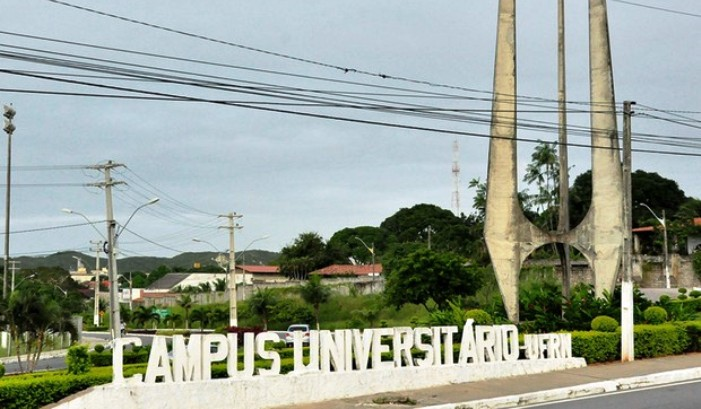
\includegraphics[width=0.95\linewidth]{internos/textuais/capitulo3-procedimentos-e-metodos/descricao-procedimento/figuras/UFRN-entrada.jpg}}
      \source{Internet}
      \label{Fig:exemplo2}
    \end{center}
\end{figure}
\paragrafo{}
Texto Texto Texto Texto Texto Texto Texto Texto Texto Texto Texto Texto Texto Texto Texto Texto Texto Texto Texto Texto Texto Texto Texto Texto Texto Texto Texto Texto Texto Texto Texto Texto Texto Texto Texto Texto Texto Texto Texto Texto Texto Texto.
\paragrafo{}
Texto Texto Texto Texto Texto Texto Texto Texto Texto Texto Texto Texto Texto Texto Texto Texto Texto Texto Texto Texto Texto Texto Texto Texto Texto Texto Texto Texto Texto Texto Texto Texto Texto Texto Texto Texto Texto Texto Texto Texto Texto Texto.
\paragrafo{}
Texto Texto Texto Texto Texto Texto Texto Texto Texto Texto Texto Texto Texto Texto Texto Texto Texto Texto Texto Texto Texto Texto Texto Texto Texto Texto Texto Texto Texto Texto Texto Texto Texto Texto Texto Texto Texto Texto Texto Texto Texto Texto.
\paragrafo{}
Texto Texto Texto Texto Texto Texto Texto Texto Texto Texto Texto Texto Texto Texto Texto Texto Texto Texto Texto Texto Texto Texto Texto Texto Texto Texto Texto Texto Texto Texto Texto Texto Texto Texto Texto Texto Texto Texto Texto Texto Texto Texto.
\paragrafo{}
Texto Texto Texto Texto Texto Texto Texto Texto Texto Texto Texto Texto Texto Texto Texto Texto Texto Texto Texto Texto Texto Texto Texto Texto Texto Texto Texto Texto Texto Texto Texto Texto Texto Texto Texto Texto Texto Texto Texto Texto Texto Texto.
\paragrafo{}
Texto Texto Texto Texto Texto Texto Texto Texto Texto Texto Texto Texto Texto Texto Texto Texto Texto Texto Texto Texto Texto Texto Texto Texto Texto Texto Texto Texto Texto Texto Texto Texto Texto Texto Texto Texto Texto Texto Texto Texto Texto Texto.
\paragrafo{}
Texto Texto Texto Texto Texto Texto Texto Texto Texto Texto Texto Texto Texto Texto Texto Texto Texto Texto Texto Texto Texto Texto Texto Texto Texto Texto Texto Texto Texto Texto Texto Texto Texto Texto Texto Texto Texto Texto Texto Texto Texto Texto.
\paragrafo{}
Texto Texto Texto Texto Texto Texto Texto Texto Texto Texto Texto Texto Texto Texto Texto Texto Texto Texto Texto Texto Texto Texto Texto Texto Texto Texto Texto Texto Texto Texto Texto Texto Texto Texto Texto Texto Texto Texto Texto Texto Texto Texto.
\paragrafo{}
Texto Texto Texto Texto Texto Texto Texto Texto Texto Texto Texto Texto Texto Texto Texto Texto Texto Texto Texto Texto Texto Texto Texto Texto Texto Texto Texto Texto Texto Texto Texto Texto Texto Texto Texto Texto Texto Texto Texto Texto Texto Texto.
\paragrafo{}
Texto Texto Texto Texto Texto Texto Texto Texto Texto Texto Texto Texto Texto Texto Texto Texto Texto Texto Texto Texto Texto Texto Texto Texto Texto Texto Texto Texto Texto Texto Texto Texto Texto Texto Texto Texto Texto Texto Texto Texto Texto Texto.
\paragrafo{}
Texto Texto Texto Texto Texto Texto Texto Texto Texto Texto Texto Texto Texto Texto Texto Texto Texto Texto Texto Texto Texto Texto Texto Texto Texto Texto Texto Texto Texto Texto Texto Texto Texto Texto Texto Texto Texto Texto Texto Texto Texto Texto.
\paragrafo{}
Texto Texto Texto Texto Texto Texto Texto Texto Texto Texto Texto Texto Texto Texto Texto Texto Texto Texto Texto Texto Texto Texto Texto Texto Texto Texto Texto Texto Texto Texto Texto Texto Texto Texto Texto Texto Texto Texto Texto Texto Texto Texto.
\paragrafo{}
Texto Texto Texto Texto Texto Texto Texto Texto Texto Texto Texto Texto Texto Texto Texto Texto Texto Texto Texto Texto Texto Texto Texto Texto Texto Texto Texto Texto Texto Texto Texto Texto Texto Texto Texto Texto Texto Texto Texto Texto Texto Texto.

\chapter{Estudo de Caso}
% ----------------------------------------------------------
\paragrafo{}
Texto Texto Texto Texto Texto Texto Texto Texto Texto Texto Texto Texto Texto Texto Texto Texto Texto Texto Texto Texto Texto Texto Texto Texto Texto Texto Texto Texto Texto Texto Texto Texto Texto Texto Texto Texto Texto Texto Texto Texto Texto Texto.
\paragrafo{}
Texto Texto Texto Texto Texto Texto Texto Texto Texto Texto Texto Texto Texto Texto Texto Texto Texto Texto Texto Texto Texto Texto Texto Texto Texto Texto Texto Texto Texto Texto Texto Texto Texto Texto Texto Texto Texto Texto Texto Texto Texto Texto.
\paragrafo{}
Texto Texto Texto Texto Texto Texto Texto Texto Texto Texto Texto Texto Texto Texto Texto Texto Texto Texto Texto Texto Texto Texto Texto Texto Texto Texto Texto Texto Texto Texto Texto Texto Texto Texto Texto Texto Texto Texto Texto Texto Texto Texto.
\paragrafo{}
Texto Texto Texto Texto Texto Texto Texto Texto Texto Texto Texto Texto Texto Texto Texto Texto Texto Texto Texto Texto Texto Texto Texto Texto Texto Texto Texto Texto Texto Texto Texto Texto Texto Texto Texto Texto Texto Texto Texto Texto Texto Texto.
\paragrafo{}
Texto Texto Texto Texto Texto Texto Texto Texto Texto Texto Texto Texto Texto Texto Texto Texto Texto Texto Texto Texto Texto Texto Texto Texto Texto Texto Texto Texto Texto Texto Texto Texto Texto Texto Texto Texto Texto Texto Texto Texto Texto Texto.
\paragrafo{}
Texto Texto Texto Texto Texto Texto Texto Texto Texto Texto Texto Texto Texto Texto Texto Texto Texto Texto Texto Texto Texto Texto Texto Texto Texto Texto Texto Texto Texto Texto Texto Texto Texto Texto Texto Texto Texto Texto Texto Texto Texto Texto.
\paragrafo{}
Texto Texto Texto Texto Texto Texto Texto Texto Texto Texto Texto Texto Texto Texto Texto Texto Texto Texto Texto Texto Texto Texto Texto Texto Texto Texto Texto Texto Texto Texto Texto Texto Texto Texto Texto Texto Texto Texto Texto Texto Texto Texto.
\paragrafo{}
Texto Texto Texto Texto Texto Texto Texto Texto Texto Texto Texto Texto Texto Texto Texto Texto Texto Texto Texto Texto Texto Texto Texto Texto Texto Texto Texto Texto Texto Texto Texto Texto Texto Texto Texto Texto Texto Texto Texto Texto Texto Texto.
\paragrafo{}
Texto Texto Texto Texto Texto Texto Texto Texto Texto Texto Texto Texto Texto Texto Texto Texto Texto Texto Texto Texto Texto Texto Texto Texto Texto Texto Texto Texto Texto Texto Texto Texto Texto Texto Texto Texto Texto Texto Texto Texto Texto Texto.
\paragrafo{}
Texto Texto Texto Texto Texto Texto Texto Texto Texto Texto Texto Texto Texto Texto Texto Texto Texto Texto Texto Texto Texto Texto Texto Texto Texto Texto Texto Texto Texto Texto Texto Texto Texto Texto Texto Texto Texto Texto Texto Texto Texto Texto.
\paragrafo{}
Texto Texto Texto Texto Texto Texto Texto Texto Texto Texto Texto Texto Texto Texto Texto Texto Texto Texto Texto Texto Texto Texto Texto Texto Texto Texto Texto Texto Texto Texto Texto Texto Texto Texto Texto Texto Texto Texto Texto Texto Texto Texto.
\paragrafo{}
Texto Texto Texto Texto Texto Texto Texto Texto Texto Texto Texto Texto Texto Texto Texto Texto Texto Texto Texto Texto Texto Texto Texto Texto Texto Texto Texto Texto Texto Texto Texto Texto Texto Texto Texto Texto Texto Texto Texto Texto Texto Texto.
\paragrafo{}
Texto Texto Texto Texto Texto Texto Texto Texto Texto Texto Texto Texto Texto Texto Texto Texto Texto Texto Texto Texto Texto Texto Texto Texto Texto Texto Texto Texto Texto Texto Texto Texto Texto Texto Texto Texto Texto Texto Texto Texto Texto Texto.
\paragrafo{}
Texto Texto Texto Texto Texto Texto Texto Texto Texto Texto Texto Texto Texto Texto Texto Texto Texto Texto Texto Texto Texto Texto Texto Texto Texto Texto Texto Texto Texto Texto Texto Texto Texto Texto Texto Texto Texto Texto Texto Texto Texto Texto.
\paragrafo{}
Texto Texto Texto Texto Texto Texto Texto Texto Texto Texto Texto Texto Texto Texto Texto Texto Texto Texto Texto Texto Texto Texto Texto Texto Texto Texto Texto Texto Texto Texto Texto Texto Texto Texto Texto Texto Texto Texto Texto Texto Texto Texto.
\paragrafo{}
Texto Texto Texto Texto Texto Texto Texto Texto Texto Texto Texto Texto Texto Texto Texto Texto Texto Texto Texto Texto Texto Texto Texto Texto Texto Texto Texto Texto Texto Texto Texto Texto Texto Texto Texto Texto Texto Texto Texto Texto Texto Texto.
\paragrafo{}
Texto Texto Texto Texto Texto Texto Texto Texto Texto Texto Texto Texto Texto Texto Texto Texto Texto Texto Texto Texto Texto Texto Texto Texto Texto Texto Texto Texto Texto Texto Texto Texto Texto Texto Texto Texto Texto Texto Texto Texto Texto Texto.
\paragrafo{}
Texto Texto Texto Texto Texto Texto Texto Texto Texto Texto Texto Texto Texto Texto Texto Texto Texto Texto Texto Texto Texto Texto Texto Texto Texto Texto Texto Texto Texto Texto Texto Texto Texto Texto Texto Texto Texto Texto Texto Texto Texto Texto.
\paragrafo{}
Texto Texto Texto Texto Texto Texto Texto Texto Texto Texto Texto Texto Texto Texto Texto Texto Texto Texto Texto Texto Texto Texto Texto Texto Texto Texto Texto Texto Texto Texto Texto Texto Texto Texto Texto Texto Texto Texto Texto Texto Texto Texto.
\paragrafo{}
Texto Texto Texto Texto Texto Texto Texto Texto Texto Texto Texto Texto Texto Texto Texto Texto Texto Texto Texto Texto Texto Texto Texto Texto Texto Texto Texto Texto Texto Texto Texto Texto Texto Texto Texto Texto Texto Texto Texto Texto Texto Texto.
\paragrafo{}
Texto Texto Texto Texto Texto Texto Texto Texto Texto Texto Texto Texto Texto Texto Texto Texto Texto Texto Texto Texto Texto Texto Texto Texto Texto Texto Texto Texto Texto Texto Texto Texto Texto Texto Texto Texto Texto Texto Texto Texto Texto Texto.
\paragrafo{}
Texto Texto Texto Texto Texto Texto Texto Texto Texto Texto Texto Texto Texto Texto Texto Texto Texto Texto Texto Texto Texto Texto Texto Texto Texto Texto Texto Texto Texto Texto Texto Texto Texto Texto Texto Texto Texto Texto Texto Texto Texto Texto.
\paragrafo{}
Texto Texto Texto Texto Texto Texto Texto Texto Texto Texto Texto Texto Texto Texto Texto Texto Texto Texto Texto Texto Texto Texto Texto Texto Texto Texto Texto Texto Texto Texto Texto Texto Texto Texto Texto Texto Texto Texto Texto Texto Texto Texto.
\chapter{Resultados}
\paragrafo{}
Texto Texto Texto Texto Texto Texto Texto Texto Texto Texto Texto Texto Texto Texto Texto Texto Texto Texto Texto Texto Texto Texto Texto Texto Texto Texto Texto Texto Texto Texto Texto Texto Texto Texto Texto Texto Texto Texto Texto Texto Texto Texto.
\paragrafo{}
Texto Texto Texto Texto Texto Texto Texto Texto Texto Texto Texto Texto Texto Texto Texto Texto Texto Texto Texto Texto Texto Texto Texto Texto Texto Texto Texto Texto Texto Texto Texto Texto Texto Texto Texto Texto Texto Texto Texto Texto Texto Texto.
\paragrafo{}
Texto Texto Texto Texto Texto Texto Texto Texto Texto Texto Texto Texto Texto Texto Texto Texto Texto Texto Texto Texto Texto Texto Texto Texto Texto Texto Texto Texto Texto Texto Texto Texto Texto Texto Texto Texto Texto Texto Texto Texto Texto Texto.
\paragrafo{}
Texto Texto Texto Texto Texto Texto Texto Texto Texto Texto Texto Texto Texto Texto Texto Texto Texto Texto Texto Texto Texto Texto Texto Texto Texto Texto Texto Texto Texto Texto Texto Texto Texto Texto Texto Texto Texto Texto Texto Texto Texto Texto.
\paragrafo{}
Texto Texto Texto Texto Texto Texto Texto Texto Texto Texto Texto Texto Texto Texto Texto Texto Texto Texto Texto Texto Texto Texto Texto Texto Texto Texto Texto Texto Texto Texto Texto Texto Texto Texto Texto Texto Texto Texto Texto Texto Texto Texto.
\paragrafo{}
Texto Texto Texto Texto Texto Texto Texto Texto Texto Texto Texto Texto Texto Texto Texto Texto Texto Texto Texto Texto Texto Texto Texto Texto Texto Texto Texto Texto Texto Texto Texto Texto Texto Texto Texto Texto Texto Texto Texto Texto Texto Texto.
\paragrafo{}
Texto Texto Texto Texto Texto Texto Texto Texto Texto Texto Texto Texto Texto Texto Texto Texto Texto Texto Texto Texto Texto Texto Texto Texto Texto Texto Texto Texto Texto Texto Texto Texto Texto Texto Texto Texto Texto Texto Texto Texto Texto Texto.
\paragrafo{}
Texto Texto Texto Texto Texto Texto Texto Texto Texto Texto Texto Texto Texto Texto Texto Texto Texto Texto Texto Texto Texto Texto Texto Texto Texto Texto Texto Texto Texto Texto Texto Texto Texto Texto Texto Texto Texto Texto Texto Texto Texto Texto.
\paragrafo{}
Texto Texto Texto Texto Texto Texto Texto Texto Texto Texto Texto Texto Texto Texto Texto Texto Texto Texto Texto Texto Texto Texto Texto Texto Texto Texto Texto Texto Texto Texto Texto Texto Texto Texto Texto Texto Texto Texto Texto Texto Texto Texto.
\paragrafo{}
Texto Texto Texto Texto Texto Texto Texto Texto Texto Texto Texto Texto Texto Texto Texto Texto Texto Texto Texto Texto Texto Texto Texto Texto Texto Texto Texto Texto Texto Texto Texto Texto Texto Texto Texto Texto Texto Texto Texto Texto Texto Texto.
\paragrafo{}
Texto Texto Texto Texto Texto Texto Texto Texto Texto Texto Texto Texto Texto Texto Texto Texto Texto Texto Texto Texto Texto Texto Texto Texto Texto Texto Texto Texto Texto Texto Texto Texto Texto Texto Texto Texto Texto Texto Texto Texto Texto Texto.
\section{Exemplo de Tabela}
\begin{table}[H]
\IBGEtab{%
  \tiny%
  \legenda{Exemplo tabela 1}%
  \label{Tab:tabela-e1}
}{%
  \begin{tabular}{m{0.3\textwidth}m{0.2\textwidth}m{0.2\textwidth}}

  \toprule
  Exemplo 1 & Exemplo 2 & Exemplo 3 & Exemplo 4 \\
  \midrule \midrule
    1         & 1         & 1         & 2         \\
    2         & 3         & 4         & 5         \\
    44        & 2         & 1         & 2         \\
  \bottomrule
\end{tabular}%
}{%
  \fonte{Autor}%
  }
\end{table}

\section{Exemplo Quadro}
\begin{quadro}[H]
\tiny
% Please add the following required packages to your document preamble:
% \usepackage{multirow}
\legenda{Exemplo de quadro 1}
\label{Quadro:exemplo1}
\begin{tabular}{|r|l|l|l|l|l|}
\hline
Exemplo 1 & Exemplo 2 & Exemplo 3 & Exemplo 4 \\ \hline
1         & 1         & 1         & 2         \\ \hline
2         & 3         & 4         & 5         \\ \hline
44        & 2         & 1         & 2         \\ \hline
\end{tabular}
\source{Exemplo}
\end{quadro}

\chapter{Conclusão}
\paragrafo{}
Texto Texto Texto Texto Texto Texto Texto Texto Texto Texto Texto Texto Texto Texto Texto Texto Texto Texto Texto Texto Texto Texto Texto Texto Texto Texto Texto Texto Texto Texto Texto Texto Texto Texto Texto Texto Texto Texto Texto Texto Texto Texto.
\paragrafo{}
Texto Texto Texto Texto Texto Texto Texto Texto Texto Texto Texto Texto Texto Texto Texto Texto Texto Texto Texto Texto Texto Texto Texto Texto Texto Texto Texto Texto Texto Texto Texto Texto Texto Texto Texto Texto Texto Texto Texto Texto Texto Texto.
\paragrafo{}
Texto Texto Texto Texto Texto Texto Texto Texto Texto Texto Texto Texto Texto Texto Texto Texto Texto Texto Texto Texto Texto Texto Texto Texto Texto Texto Texto Texto Texto Texto Texto Texto Texto Texto Texto Texto Texto Texto Texto Texto Texto Texto.
\paragrafo{}
Texto Texto Texto Texto Texto Texto Texto Texto Texto Texto Texto Texto Texto Texto Texto Texto Texto Texto Texto Texto Texto Texto Texto Texto Texto Texto Texto Texto Texto Texto Texto Texto Texto Texto Texto Texto Texto Texto Texto Texto Texto Texto.
\paragrafo{}
Texto Texto Texto Texto Texto Texto Texto Texto Texto Texto Texto Texto Texto Texto Texto Texto Texto Texto Texto Texto Texto Texto Texto Texto Texto Texto Texto Texto Texto Texto Texto Texto Texto Texto Texto Texto Texto Texto Texto Texto Texto Texto.
\paragrafo{}
Texto Texto Texto Texto Texto Texto Texto Texto Texto Texto Texto Texto Texto Texto Texto Texto Texto Texto Texto Texto Texto Texto Texto Texto Texto Texto Texto Texto Texto Texto Texto Texto Texto Texto Texto Texto Texto Texto Texto Texto Texto Texto.
\paragrafo{}
Texto Texto Texto Texto Texto Texto Texto Texto Texto Texto Texto Texto Texto Texto Texto Texto Texto Texto Texto Texto Texto Texto Texto Texto Texto Texto Texto Texto Texto Texto Texto Texto Texto Texto Texto Texto Texto Texto Texto Texto Texto Texto.
\paragrafo{}
Texto Texto Texto Texto Texto Texto Texto Texto Texto Texto Texto Texto Texto Texto Texto Texto Texto Texto Texto Texto Texto Texto Texto Texto Texto Texto Texto Texto Texto Texto Texto Texto Texto Texto Texto Texto Texto Texto Texto Texto Texto Texto.
\paragrafo{}
Texto Texto Texto Texto Texto Texto Texto Texto Texto Texto Texto Texto Texto Texto Texto Texto Texto Texto Texto Texto Texto Texto Texto Texto Texto Texto Texto Texto Texto Texto Texto Texto Texto Texto Texto Texto Texto Texto Texto Texto Texto Texto.
\paragrafo{}
Texto Texto Texto Texto Texto Texto Texto Texto Texto Texto Texto Texto Texto Texto Texto Texto Texto Texto Texto Texto Texto Texto Texto Texto Texto Texto Texto Texto Texto Texto Texto Texto Texto Texto Texto Texto Texto Texto Texto Texto Texto Texto.
\paragrafo{}
Texto Texto Texto Texto Texto Texto Texto Texto Texto Texto Texto Texto Texto Texto Texto Texto Texto Texto Texto Texto Texto Texto Texto Texto Texto Texto Texto Texto Texto Texto Texto Texto Texto Texto Texto Texto Texto Texto Texto Texto Texto Texto.

% ----------------------------------------------------------
% ELEMENTOS PÓS-TEXTUAIS
% ----------------------------------------------------------
\postextual
% ----------------------------------------------------------
% ----------------------------------------------------------
% Referências bibliográficas
% ----------------------------------------------------------

\bibliography{bibliografia/bibliografia}
%
% Consulte o manual da classe abntex2 para orientações sobre o glossário.
%
%\glossary
% ----------------------------------------------------------
% Apêndices
% ----------------------------------------------------------
% ---
% Inicia os apêndices
% ---
\begin{apendicesenv}
% Imprime uma página indicando o início dos apêndices
\partapendices
% ----------------------------------------------------------
\chapter{Exemplo apendice}
\label{Apndx:apendice-entrevista}
\Large Entrevista Semiestruturada 
\normalsize
\begin{itemize}
    \item Explicação da pesquisa
    \begin{itemize}
        \item Tópico 1;
        \item Tópico 2;
        \item Tópico 3;
        \item Tópico 4;
        \item Tópico 5;
        \item Tópico 6;
        \item Tópico 7;
    \end{itemize}
\end{itemize}
\end{apendicesenv}
% ---
% ----------------------------------------------------------
% Anexos
% ----------------------------------------------------------
% ---
% Inicia os anexos
% ---
\begin{anexosenv}
% Imprime uma página indicando o início dos anexos
\partanexos
% ---
\chapter{Morbi ultrices rutrum lorem.}
% ---
\lipsum[30]
% ---
\chapter{Cras non urna sed feugiat cum sociis natoque penatibus et magnis dis
parturient montes nascetur ridiculus mus}
% ---
sss
% ---
\chapter{Fusce facilisis lacinia dui}
% ---
\lipsum[32]
\end{anexosenv}
%---------------------------------------------------------------------
% INDICE REMISSIVO
%---------------------------------------------------------------------
%\phantompart
\printindex
%---------------------------------------------------------------------
\end{document}
